\documentclass[12pt]{article}
\usepackage{graphics,textcomp}
\newcommand{\micro}{\hbox{\textmu}}
\newcommand{\unit}[1]{\mathrm{#1}}
  \renewcommand{\deg}{\unit{deg}}
  \newcommand{\rad}{\unit{rad}}
  \newcommand{\s}{\unit{s}}
  \newcommand{\ns}{\unit{ns}}
  \newcommand{\m}{\unit{m}}
  \newcommand{\fm}{\unit{fm}}
  \newcommand{\mps}{\m\,\s^{-1}}
  \newcommand{\cm}{\unit{cm}}
  \newcommand{\mm}{\unit{mm}}
  \newcommand{\mum}{\unit{\micro m}}
  \newcommand{\nm}{\unit{nm}}
  \newcommand{\kg}{\unit{kg}}
  \newcommand{\Hz}{\unit{Hz}}
  \newcommand{\N}{\unit{N}}
  \newcommand{\J}{\unit{J}}
  \newcommand{\W}{\unit{W}}
  \newcommand{\A}{\unit{A}}
  \newcommand{\F}{\unit{F}}
\newcounter{answer}
\newenvironment{alist}{\begin{list}{(\Alph{answer})}{\usecounter{answer}}}%
  {\end{list}}
\newcommand{\explicitcorrect}[1]{[({#1})~\textbf{correct}]}
\newcommand{\correct}{~[\textbf{correct}]}
\newcommand{\source}[1]{\textsl{(from {#1})}}
\renewcommand{\emph}[1]{\textbf{#1}}
\begin{document}
\raggedright
\begin{enumerate}

\item \source{lecture 2009-01-21} The fundamenal frequency of a piano
  string is $400\,\Hz$.  It is $1\,\m$ long.  Which of the following
  is closest to the wave speed in this piano string?
  \begin{alist}
  \item $0.0025\,\m\,\s^{-1}$
  \item $0.005\,\m\,\s^{-1}$
  \item $200\,\m\,\s^{-1}$
  \item $400\,\m\,\s^{-1}$
  \item $800\,\m\,\s^{-1}$\correct
  \end{alist}

\item \source{lecture 2009-01-26} What are the units of the ratio
  $P/\rho$, where $P$ is pressure and $\rho$ is density?
  \begin{alist}
  \item $\J\,\m^{-3}$
  \item $\kg\,\m^{-3}$
  \item $\N\,\kg^{-3}$
  \item $\m^2\,\s^{-2}$\correct
  \item none of the above
  \end{alist}

\item \source{exam~1} Two loudspeakers, A and B, are driven by
  the same amplifier and emit sinusoidal waves in phase. The frequency
  of the waves emitted by each speaker is $172\,\Hz$. You are
  $4.00\,\m$ from speaker A. Take the speed of sound in air to be
  $344\,\mps$.  What is the closest you can be to speaker B and be at
  a point of destructive interference?\begin{alist}
    \item $0.25\,\m$
    \item $0.50\,\m$
    \item $1.00\,\m$\correct
    \item $1.50\,\m$
    \item $2.00\,\m$
  \end{alist}

\item \source{exercise 21.24} A very thin oil film ($n=1.25$) floats
  on water ($n=1.33$).  What is the thinnest film that produces strong
  reflection of green light with wavelength of $500\,\nm$?
  \begin{alist}
  \item $125\,\nm$
  \item $200\,\nm$\correct
  \item $250\,\nm$
  \item $400\,\nm$
  \item $500\,\nm$
  \end{alist}

\item \source{exercise 23.14} An underwater (water has $n=1.33$) diver
  sees the sun 60\,degrees above the horizontal.  How high is the sun
  above the horizontal for a fisherman out of the water?
  \begin{alist}
  \item 22\,degrees
  \item 42\,degrees
  \item 48\,degrees\correct
  \item 68\,degrees
  \item not possible; there is total internal reflection
  \end{alist}

\item \source{exam~1} Consider a simple camera with one
  converging lens of focal length $3.00\,\cm$ with a CCD behind it.
  If you are focusing on an object a distance $400\,\cm$ away, at what
  distance from the lens should you put the CCD to capture the image
  in focus?\begin{alist}
    \item a lot closer than $3.00\,\cm$
    \item a bit closer than $3.00\,\cm$
    \item at exactly $3.00\,\cm$
    \item a bit farther than $3.00\,\cm$\correct
    \item a lot farther than $3.00\,\cm$
  \end{alist}

\item \source{exam~2} An ion of charge $-3\,e$ and positron of charge
  $+e$ are in an evacuated part of outer space, instantaneously
  separated by a distance of $1\,\cm$.  Where is there a position at
  which a \emph{nearby} test charge would experience no electrical
  force at this moment in time?
  \begin{alist}
  \item There is a location \emph{not} between the two charges, closer
    to the positron than the ion.\correct
  \item There is a location \emph{not} between the two charges, closer
    to the ion than the positron.
  \item There is a location and it is in between the two charges.
  \item There is no such location.
  \end{alist}

\item \source{conceptual question 29.6} Which of the dipoles a, b, c,
  d, or e (you can ignore dipole f) has the \emph{lowest} potential
  energy?
  \\ \resizebox{0.75\textwidth}{!}{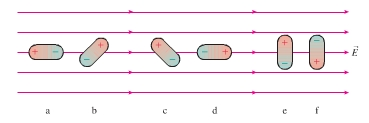
\includegraphics{dipoles.jpg}}
  \\ \explicitcorrect{D}

\item \source{exam~2} A charge $q$ of mass $m$ is moving initially at
  speed $v_y$ in the $y$ direction.  It passes through a uniform
  electric field $E$ acting in the $x$ direction.  This electric field
  exists only in a region of space of $y$-direction length $L$.  What
  is the $x$-direction velocity component $v_x$ after it has passed
  through this field?
  \begin{alist}
  \item $0$
  \item $\displaystyle 2\,\frac{m}{q}\,\left[\frac{v_y}{L}\right]^2$
  \item $\displaystyle\frac{L}{v_y}$
  \item $\displaystyle\frac{q\,E\,L}{m\,v_y}$\correct
  \item none of the above
  \end{alist}

\item \source{lecture 2009-03-23} What is the mean current (roughly) for
  a $250\,\W$ vacuum cleaner plugged into a standard North American
  outlet?
  \begin{alist}
  \item $0.2\,\A$
  \item $2\,\A$\correct
  \item $20\,\A$
  \item $200\,\A$
  \item $2000\,\A$
  \end{alist}

\item \source{exam~3} How many free electrons (roughly) are there in a
  kilogram of Copper?  (Hint: In lecture we considered the size of an
  atom, but Avogadro's number $6\times 10^{23}$ could be just as
  useful; Copper has atomic weight 64, roughly.)
  \begin{alist}
  \item $10^{19}$
  \item $10^{22}$
  \item $10^{25}$\correct
  \item $10^{28}$
  \item $10^{31}$
  \end{alist}

\item \source{lecture 2009-04-01} I have a circuit with a resistance of
  1\,ohm and a capacitance $C$.  If I want the capacitance to discharge
  in \emph{less than} 1 micro-second, then I should choose a
  capacitance
  \begin{alist}
  \item $C < 10^{-6}\,F$\correct
  \item $C > 10^{-6}\,F$
  \item $C < 10^6\,\F$
  \item $C > 10^6\,\F$
  \end{alist}

\item \source{exam~3} Two resistors made of the same material have
  different lengths but the same cross-sectional area $A$.  Resistor
  $R_1$ has length $\ell$ and resistor $R_2$ has length $2\,\ell$.
  Each resistor has the same voltage $V$ applied to it.  Which
  statement is closest to true?
  \begin{alist}
  \item Resistor $R_1$ has a larger internal electric field and a larger internal current density than resistor $R_2$.\correct
  \item Resistor $R_1$ has a smaller internal electric field and a larger internal current density than resistor $R_2$.
  \item Resistor $R_1$ has a larger internal electric field and a smaller internal current density than resistor $R_2$.
  \item Resistor $R_1$ has a smaller internal electric field and a smaller internal current density than resistor $R_2$.
  \item The two resistors have the same internal electric field and the same internal current density.
  \end{alist}

\item \source{exercise 32.21} A resistor of resistance $R$ is in
  parallel to a resistor of 200\,ohm.  To what should you set $R$ to
  get a total effective resistance of 150\,ohm?
  \begin{alist}
  \item 30\,ohm
  \item 50\,ohm
  \item 100\,ohm
  \item 400\,ohm
  \item 600\,ohm\correct
  \end{alist}

\item \source{lecture 2009-04-13} A beam of electrons in a cathode-ray
  is traveling in the northward direction, and a magnetic field is applied
  in the upwards direction.  In what direction is the beam deflected?
  \begin{alist}
  \item north
  \item east
  \item south
  \item west\correct
  \end{alist}

\item \source{lecture 2009-04-15} The bar in the diagram shown (below)
  moves at speed $v$ through a magnetic field of magnitude $B$
  pointing out of the page.  The bar has length $L$.  What is the
  voltage generated across the bar?
  \\ \resizebox{0.25\textwidth}{!}{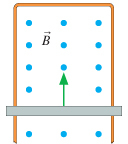
\includegraphics{34_Q01.jpg}}
  \begin{alist}
  \item $\displaystyle\frac{v\,B}{\mu_0\,L}$
  \item $\displaystyle\frac{2\,\pi\,B\,L}{\mu_0}$
  \item $v\,B\,L$\correct
  \item $v\,E\,L$
  \item can't answer without the resistivity $\rho$
  \end{alist}

\item \source{lecture 2009-04-20} A loop of wire is thrown upwards
  from a region of zero magnetic field into a region of high magnetic
  field pointing out of the page as shown below.  As it enters the
  field, the loop obtains an induced current and feels a force.
  \\ \resizebox{0.25\textwidth}{!}{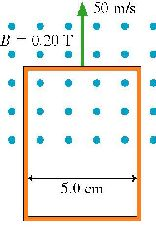
\includegraphics{knight_Figure_33_12.jpg}}
  \begin{alist}
  \item The current is clockwise and the force is downwards.\correct
  \item The current is clockwise and the force is upwards.
  \item The current is counter-clockwise and the force is downwards.
  \item The current is counter-clockwise and the force is upwards.
  \end{alist}

\item \source{exercise 38.10} What is the potential energy of two
  protons separated by 15\,fm ($1\,\fm = 10^{-15}\,\m$), to order of
  magnitude?
  \begin{alist}
  \item 0.1\,meV
  \item 0.1\,eV
  \item 0.1\,keV
  \item 0.1\,MeV\correct
  \item 0.1\,GeV
  \end{alist}

\item \source{lecture 2009-04-27} The units of Planck's constant $h$ are
  those of
  \begin{alist}
  \item energy
  \item momentum
  \item position
  \item time
  \item angular momentum\correct
  \end{alist}

\item \source{exercise 39.11} An FM radio station broadcasts at 6\,kW
  at 101\,MHz.  To within a factor of 10, how many photons does its
  antenna emit per second?
  \begin{alist}
  \item $10^{26}$
  \item $10^{27}$
  \item $10^{28}$
  \item $10^{29}$\correct
  \item $10^{30}$
  \end{alist}

\end{enumerate}
\end{document}
